\section{Parallelisation}

\begin{figure}[!h]
        \begin{center}
	\begin{subfigure}{0.45\linewidth}
		\centering
		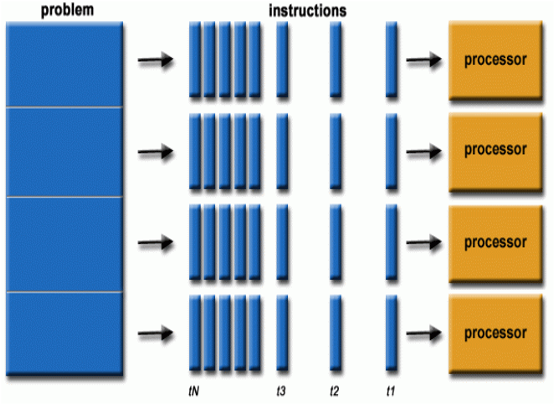
\includegraphics[width=\linewidth]{parallel_fig/parallel1.png}
	\end{subfigure}
	\begin{subfigure}{0.45\linewidth}
		\centering
		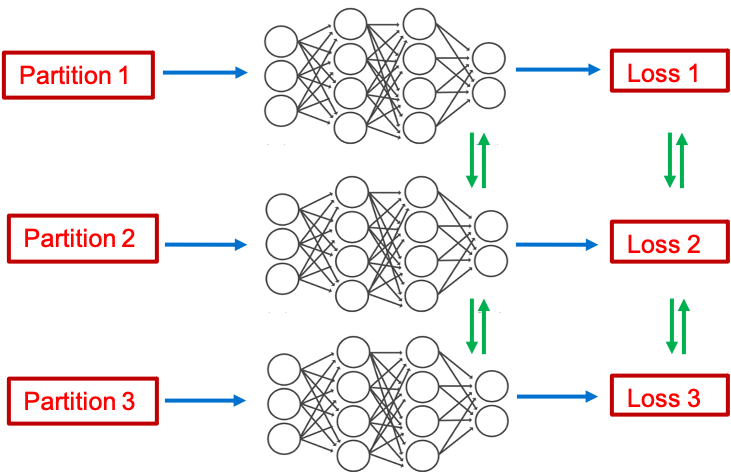
\includegraphics[width=\linewidth]{parallel_fig/parallel2.png}
	\end{subfigure}
	\caption{Parallel computing and its application in training an NN}
	\label{fig: parallel}
        \end{center}
\end{figure}

Parallelisation refers to the technique of breaking down a task into smaller subtasks that can be executed simultaneously or in parallel by multiple processing units. These processing units could be CPU cores within a single processor, multiple processors within a computer, or even distributed computing resources across a network. The goal of parallelisation is to speed up the execution of a task by distributing the workload across multiple processing units, thereby reducing the overall execution time. This is particularly useful for computationally intensive tasks divided into independent or loosely coupled subtasks. In this project, we utilised both GPU and CPU parallelisation to speed up the process of training the ANN and the process of performing POD and generating training data. 

\subsection{CPU-parallelisation}

\subsection{GPU-parallelisation}

\newpage
